\chapter{Výpočetní část}

\section{Tvorba geometrie}

Výpočetní doména byla vytvořena v programu Ansys DesignModeler podle geometrie uvedené v kapitole \ref{chap:exp}. Výsledná nestrukturovaná síť byla tvořena šestistěnnými a čtyřstěnnými buňkami o celkovém počtu \num{264398}. Průměrný objem buňky činil \SI{0.07}{\milli\litre} a průměrný skewness faktor \num{0.162}. Výpočetní doména je znázorněna na obr. \ref{fig:geo}, kde zelenou barvou je znázorněna rotační zóna kolem míchadla. 

\begin{figure}[h!]
\begin{center}
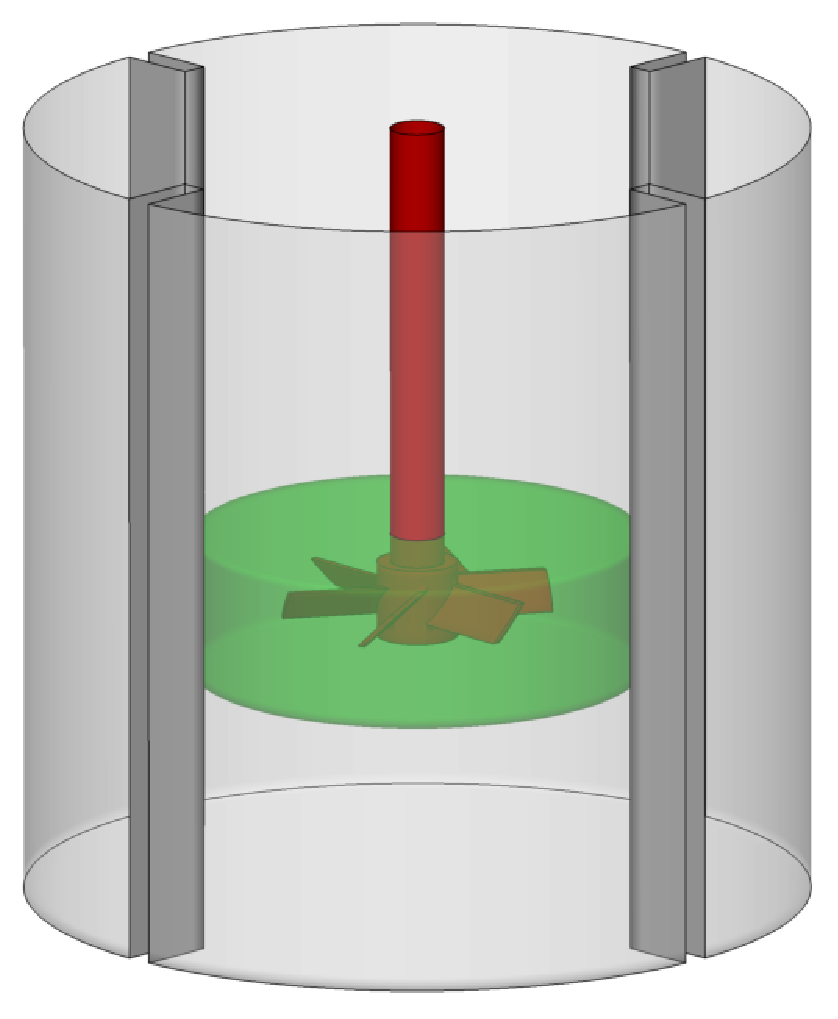
\includegraphics[scale=0.28]{images/geo.eps}
\caption{Výpočetní doména}
\label{fig:geo}
\end{center}
\end{figure} 

\section{Uživatelsky definové funkce}
Uživatelem definované funkce (UDF) jsou moduly načítané do softwaru \flu, jenž rozšiřují nebo upravují schopnosti řešiče. Například může se jednat o definovaní vlastních počátečních a okrajových podmínek, změnu materiálových vlastností a modifikaci simulačních modelů. Pro tvorbu zdrojových souborů se využívá programovací jazyk C, které jsou následně zkompilovaný do dynamické knihovny.

Všechny korelace pro odporový koeficient uvedené v tab. \ref{tab:cds} byly implementovány v podobě uživatelsky definovaných funkcí a jejich zdrojové kódy jsou uvedeny v kapitole Příloha.

\section{Vlastní CFD simulace}
K CFD simulaci byl využit komerční software \flu 12.1.4 do kterého byla načtena vytvořená výpočetní síť. Množství pevné fáze v míchací nádobě bylo zvoleno 5\,\%\,obj. pro všechny provedené výpočty. Jako vsádka byla zvolena kapalina PVP\,5, jejiž vlastnosti jsou uvedeny v tab. \ref{tab:fyzvlast}. Pohyb míchadla byl simulován pomocí metody rotující sítě (sliding mesh) a jeho rychlost otáčení byla zvolena \SI{7}{\per\second}. Model Eulerian-Eulerian byl vybrán l simulaci vícefázového proudění a pro popis turbulentního proudění byl využit standardní $k\mbox{-}\epsilon$ model s disperzní modifikací . Časový krok nestacionární simulace byl zvolen \num{0.001} sekundy. Postupně byly využity všechny korelace pro odporový koeficient uvedeny v tab. \ref{tab:cds} spolu s klasickým Schillerovým-Naumannovým vztahem. 

Simulace probíhala na počítači HP Z600 osazený dvěma procesory Intel Xeon X5570 a pamětí 24 GB s operačním systémem CentOS 5.3 x86-64. Doba výpočtu jedné reálné vteřiny trvala přibližně 3 hodiny.


